We now analyze the information-leakage of the channels corresponding to the protocols.
Recall that the smaller the capacity of a channel (c.f.r. Section~\ref{sec:prelqif}), 
the less information an adversary will obtain about the secret by observing the 
output of that channel, and the safer, hence, the channel is considered.

\subsection{\label{sec:analdin} Analyses of the Dining Cryptographers}

We implemented both variations of the Dining cryptographers for 
5, 6, 7, 8, and 9 cryptographers. 
Our results suggest the complete-DC variation is safer than the cycle-DC variation, 
yielding smaller values for all capacities measured.

\subsubsection{Results for multiplicative capacities%
% $\mathcal{L}_\forall\hyperc{\pi}{C}$ and $\mathcal{L}_\forall\hyperc{\forall}{C}$
.}

It has been proven \cite{addmult} that the multiplicative capacity
$\mathcal{L}_\forall\hyperc{\pi}{C}$ (which quantifies over all gain-functions $g$ for
a fixed prior $\pi$) collapses into the multiplicative capacity 
$\mathcal{L}_\forall\hyperc{\forall}{C}$ (which quantifies over all priors and gain-functions)
when the prior $\pi$ has full-support. 
Since we consider any cryptographer can be the payer, the prior has full support, 
and we can focus only on the latter capacity, which can be computed as follows.

\begin{Theorem}[\cite{capacity}]
\label{capacity}
Given channel $C{:}\calx{\times}\caly{\rightarrow}\reals$,
$\mathcal{L}_\forall\hyperc{\forall}{C}{=}\log \sum_{y \in \caly}\max\limits_{x \in \calx} C(x,y).$
\end{Theorem}

Figure~\ref{figure:dingraph} shows the values of this capacity for both 
variants of the DC protocol, and varying values of the probability $p$ 
of heads. 
Note that the graph of capacity must be symmetric w.r.t. $p=0.5$, 
for a coin with probability of heads $1{-}p$ is nothing more than a 
coin with probability of tails $p$.

\begin{figure}[ht]
\centering
\begin{subfigure}[b]{0.45\linewidth}
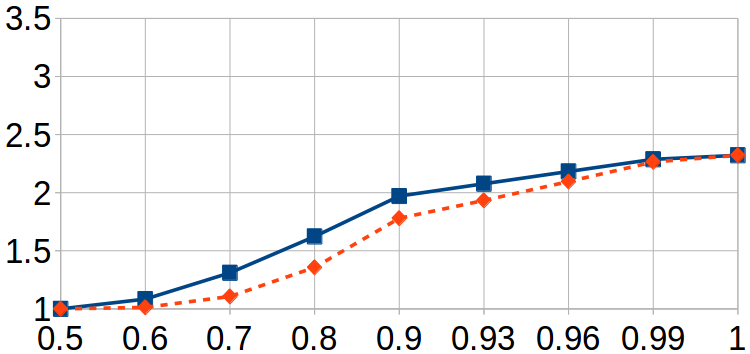
\includegraphics[width=\textwidth]{figures/dining-mult-4.png}
\caption{$\mathcal{L}_\forall\hyperc{\forall}{C}$, 4 cryptographers.}
\end{subfigure}
\hfill
\centering
\begin{subfigure}[b]{0.45\linewidth}
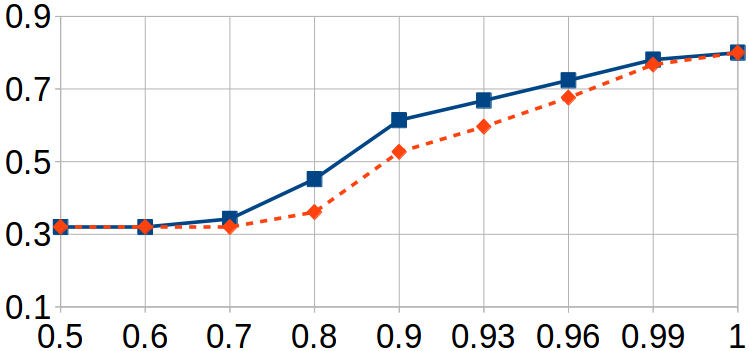
\includegraphics[width=\textwidth]{figures/dining-add-4.png}
\caption{$\mathcal{L}^+_\forall\hyperc{\pi_u}{C}$, 4 cryptographers.}
\end{subfigure}
\\ \vspace{3mm}
\begin{subfigure}[b]{0.45\linewidth}
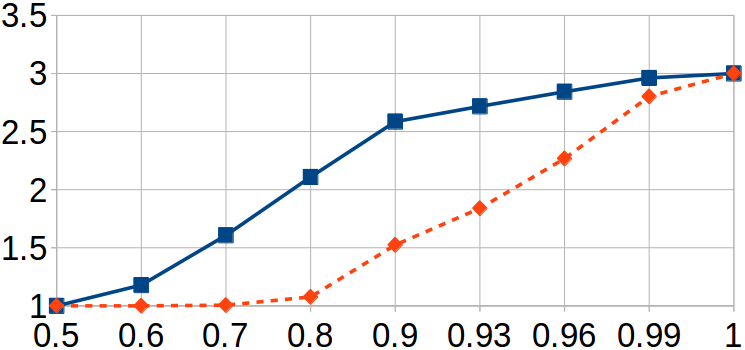
\includegraphics[width=\textwidth]{figures/dining-mult-7.png}
\caption{$\mathcal{L}_\forall\hyperc{\forall}{C}$, 7 cryptographers.}
\end{subfigure}
\hfill
\centering
\begin{subfigure}[b]{0.45\linewidth}
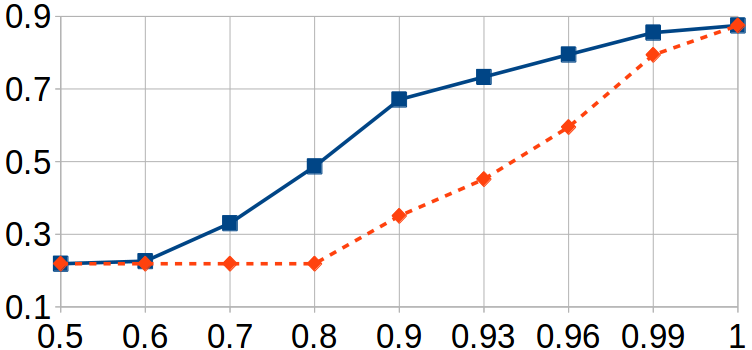
\includegraphics[width=\textwidth]{figures/dining-add-7.png}
\caption{$\mathcal{L}^+_\forall\hyperc{\pi_u}{C}$, 7 cryptographers.}
\end{subfigure}
\\ \vspace{3mm}
\begin{subfigure}[b]{0.45\linewidth}
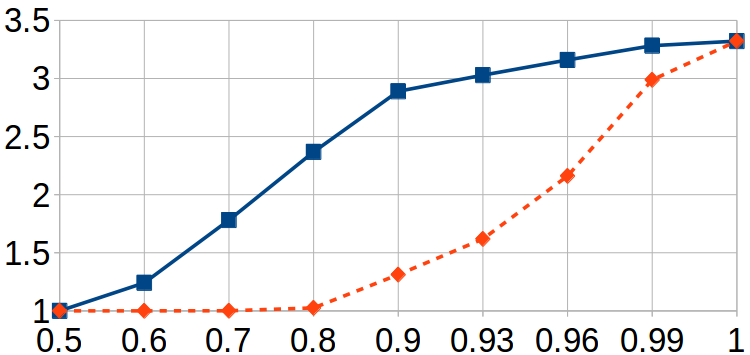
\includegraphics[width=\textwidth]{figures/dining-mult-9.png}
\caption{$\mathcal{L}_\forall\hyperc{\forall}{C}$, 9 cryptographers.}
\end{subfigure}
\hfill
\centering
\begin{subfigure}[b]{0.45\linewidth}
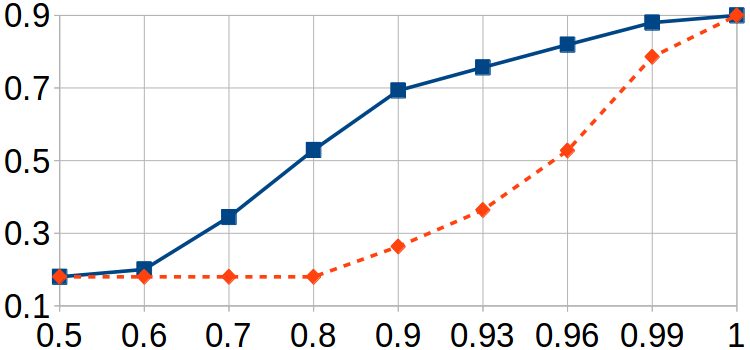
\includegraphics[width=\textwidth]{figures/dining-add-9.png}
\caption{$\mathcal{L}^+_\forall\hyperc{\pi_u}{C}$, 9 cryptographers.}
\end{subfigure}
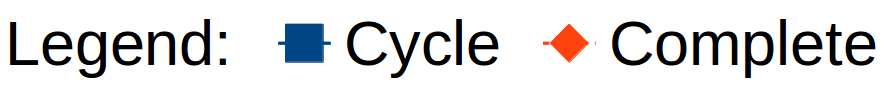
\includegraphics[width=0.3\textwidth]{figures/dining-legend.png}
\caption{Capacities for both variations of the Dining Cryptographers,
and different probabilities of heads.
The $x$-axis, for the value of probability, is \emph{not} in scale.}
\label{figure:dingraph}
\end{figure}

\review{Note} also that in all instances of both variations, 
the minimum capacity is 1, and occurs at $p=0.5$.
This reflects the fact that, if the coins are \review{fair}, the only information 
leaked is whether the NSA is paying the bill.
When $p=1$, however, all coin tosses yield heads, and any observer 
can deduce with certainty who is paying the bill from the announcements 
of the cryptographers. 
In this case the capacity reaches its maximum, being $\log (n+1)$ for 
$n$ cryptographers, for the outputs of the protocol always reveal 
the payer's identity.

\commentM{Capacity is 1 because Theorem~\ref{capacity} says it coincides with
min-capacity.
Should we interpret this result here?}
%\commentM{Also, the $x$-axes start from 0.5. We have to explain why
%(because capacity is symmetric w.r.t. that value).}

It is clear from the graph that the complete variation leaks less than the cycle one. 
Also, while the capacity of the cycle variation increases rapidly even when $p$ approaches
$0.5$, the complete variation is less susceptible to these small changes, 
maintaining information leakage close to 0.

\subsubsection{Results for additive capacity%
%$\mathcal{L}^+_\forall\hyperc{\pi}{C}$
.}
The additive capacity $\mathcal{L}^+_\forall\hyperc{\pi}{C}$ (quantifying
over all gain functions $g$, for a given prior $\pi$) can be
computed by
$ 
\mathcal{L}^+_\forall\hyperc{\pi}{C}=\sum_{x,y} \pi(x) |C(x,y) - \sum_{x'}\pi(x')C(x',y)|
$
~\cite{addmult}.
Note that, unlike its multiplicative counterpart, this capacity actually depends on 
the prior $\pi$. 

Figure~\ref{figure:dingraph} shows the values for this capacity for an uniform prior $\pi_u$, 
and varying probabilities $p$ of heads. 
The graphs confirm that the minimum and maximum values of information leakages occur, 
respectively, for $p=0.5$ and $p=1$.
We can see that complete-DC is always more secure than cycle-DC,
and its capacity keeps almost unaltered until $p$ deviates substantially from $0.5$.

\subsection{Analyses of Crowds}

We implemented both variants of the Crowds protocol for 9 users, 
and from 1 up to 3 corrupted users. 

In particular, in grid-Crowds, we need to consider another variable: the position 
of the corrupt users makes a great difference in the channels' capacities.
Figure~\ref{figure:positions} shows all possible 
positions for three corrupt users on a 3x3 grid, up to symmetry. 
(Recall that the edges going off the grid connect at opposite 
sides---e.g., user 1 can communicate with user 3 and with user 7.)
If, for instance, the corrupt users are 1,2 and 3, each 
honest user would be connected to only one corrupt user. 
If the corrupt were 1,5 and 9, however, each honest user would be 
connected to two corrupt ones. 
Therefore, the chance that the initiator will 
forward a message directly to a corrupt user is 20\% on the first scenario, 
and 40\% on the second one (please recall that the initiator may send the 
message to itself). 
Thus, it is natural to expect that the capacities for the former
will be smaller than for the latter.

\begin{figure}[ht]
\centering
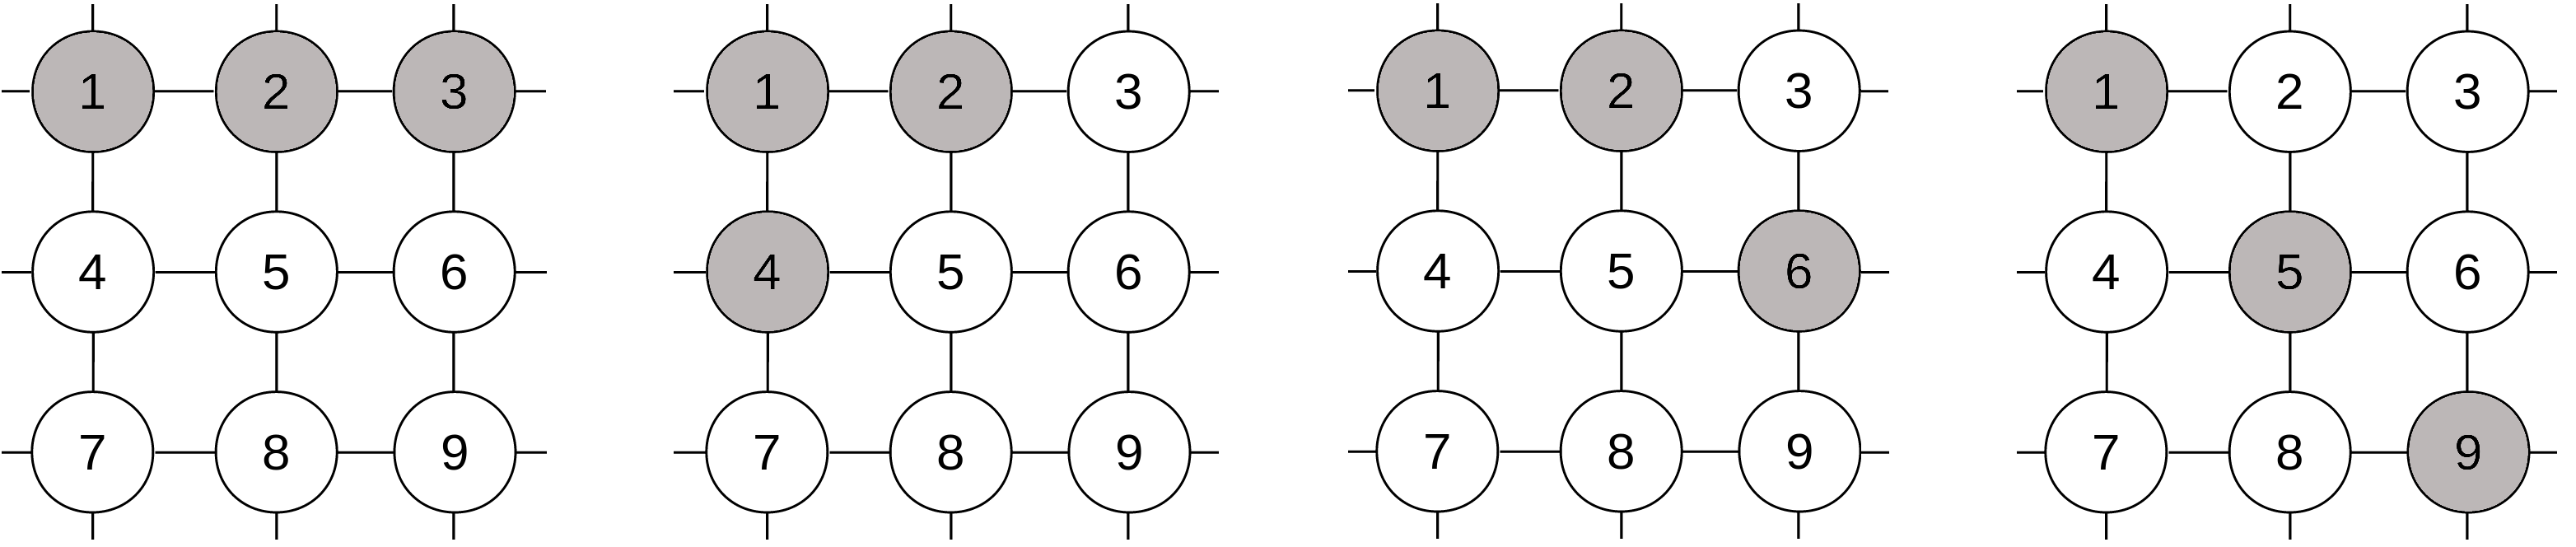
\includegraphics[width=0.8\textwidth]{figures/positions.png}
\caption{All positions (up to symmetry) for three corrupted users (colored in dark) on a 3x3 grid. }
\label{figure:positions}
\end{figure}

\subsubsection{Results for multiplicative capacities%
%$\mathcal{L}_\forall\hyperc{\pi}{C}$ and $\mathcal{L}_\forall\hyperc{\forall}{C}$
.}

We compute $\mathcal{L}_\forall\hyperc{\forall}{C}$ using Theorem~\ref{capacity}. 
Figure~\ref{figure:crgraph} shows the corresponding values for 9 users, both in 
original DC and in grid-DC.
Note that the probability $p_f$ of forwarding does not influence multiplicative 
capacity in the original DC, which confirms a known result from the literature 
\cite{minresource}.
%\commentA{Is the capacity supposed to not vary in relation to $p_f$? 
%I was not expecting this}
%\replyM{Yes, it is expected! We should give a reference to a study that shows why.
%Kostas has some paper on this, and I think Geoffrey too.} 
%\replyA{Found a proof in Geoffrey's min leakage paper}
However, we can see that it does for the grid variation. 
To understand this, notice that even if the originator does not forward 
the message to a corrupt user at first, his immediate neighbors are more 
likely to receive the message than the users he cannot communicate with. 
For example, if user 8 is detected in the 3x3 grid, it is more probable 
that the originator was user 7 than user 4.
Therefore, as the expected number of interactions between users decreases 
with $p_f$, the more likely it is that a message is detected \review{by a corrupt user or} forwarded 
to the server near its originator.

%\begin{figure}[ht]
%\centering
%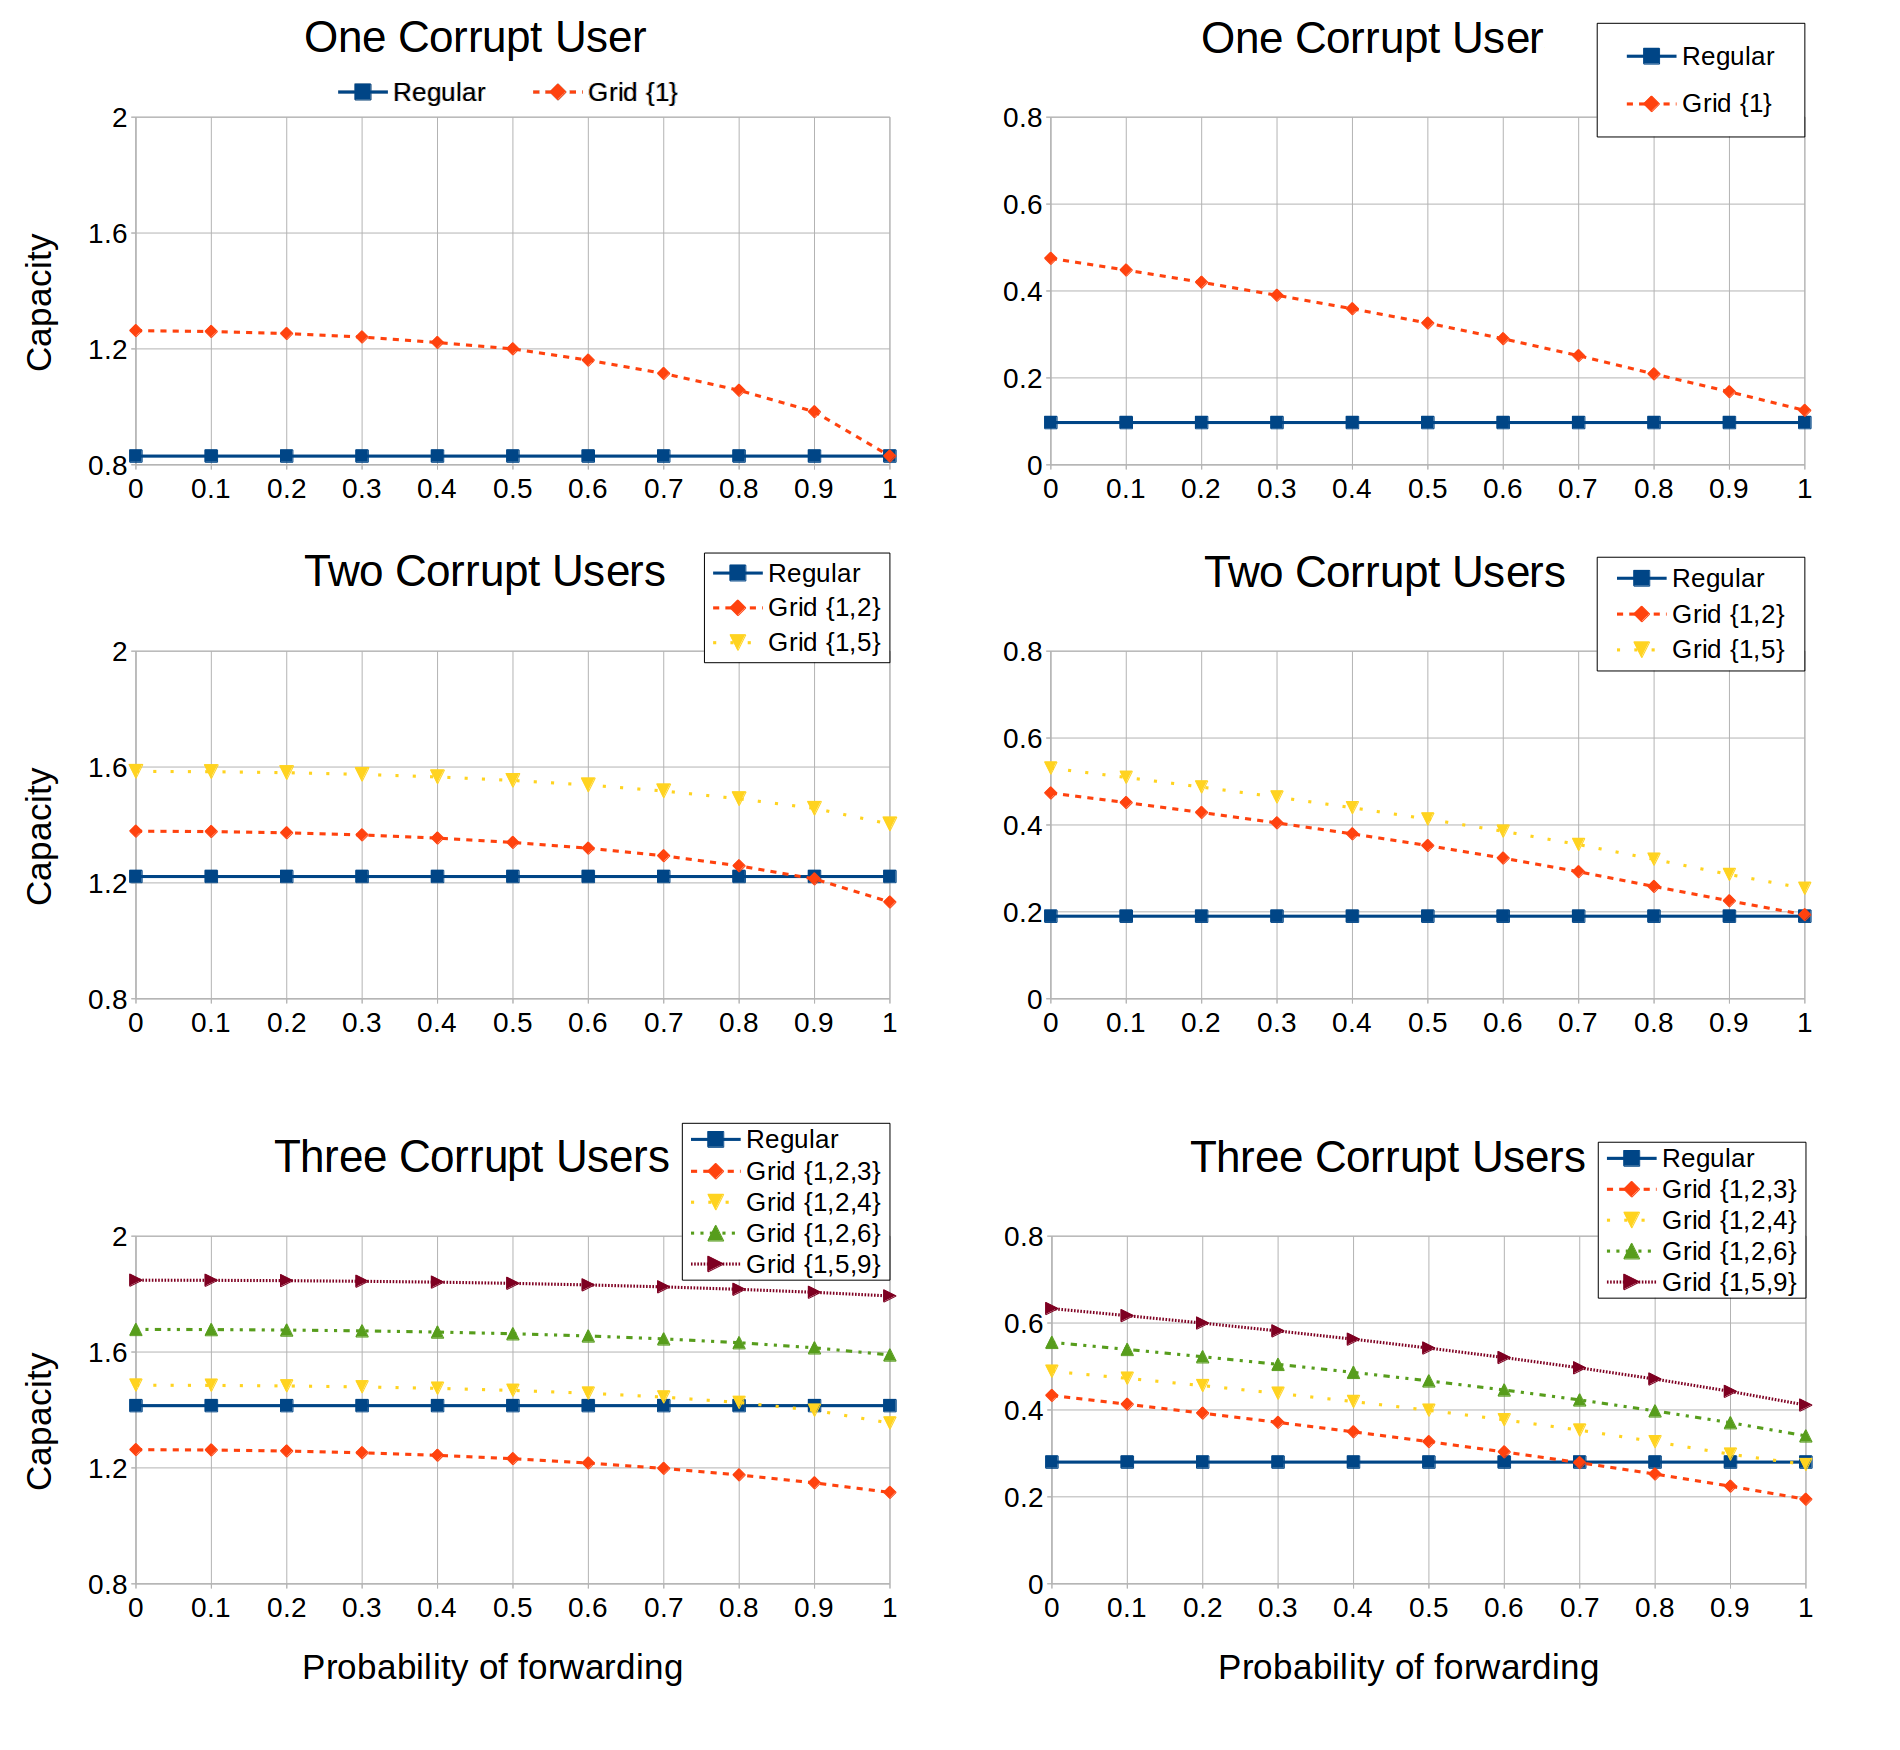
\includegraphics[width=\textwidth]{figures/crowds.png}
%\caption{Values of $\mathcal{L}_\forall\hyperc{\forall}{C}$ (left side) and
%$\mathcal{L}^+_\forall\hyperc{\pi_u}{C}$ (right side) for 9 users on both variations of the Crowds, 
%and varying number of corrupt users.
%The numbers in braces in the legends indicate the positions of the corrupt users}
%\label{figure:crgraph}
%\end{figure}

\begin{figure}[ht]
\centering
\begin{subfigure}[b]{0.45\linewidth}
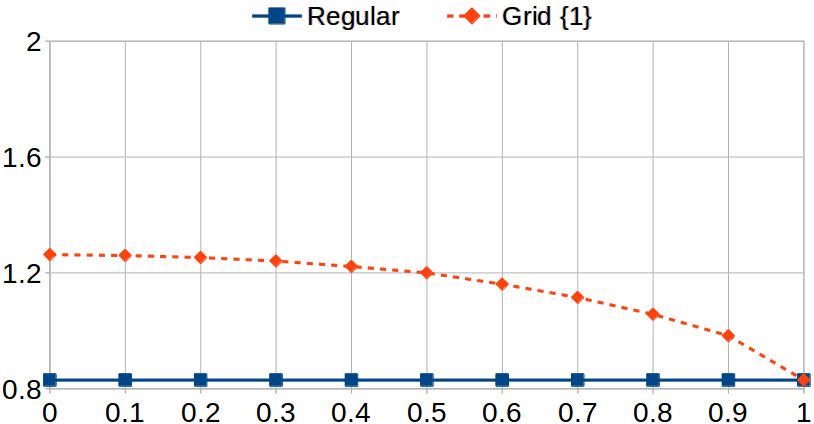
\includegraphics[width=\textwidth]{figures/crowds-mult-1.png}
\caption{$\mathcal{L}_\forall\hyperc{\forall}{C}$, 1 corrupted user.}
\end{subfigure}
\hfill
\centering
\begin{subfigure}[b]{0.45\linewidth}
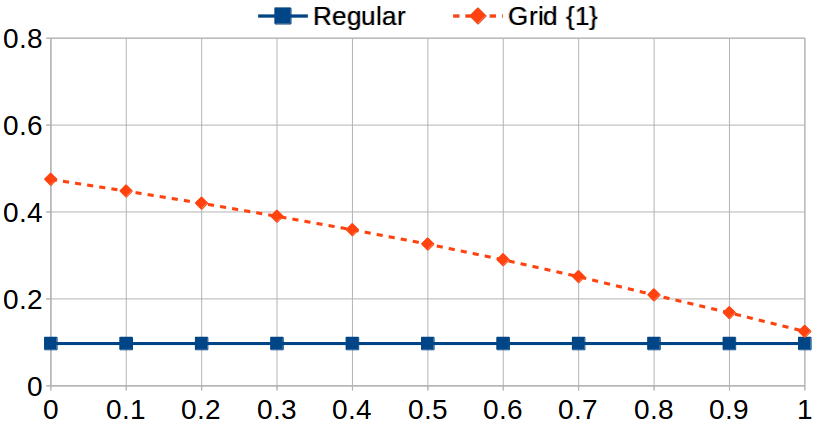
\includegraphics[width=\textwidth]{figures/crowds-add-1.png}
\caption{$\mathcal{L}^+_\forall\hyperc{\pi_u}{C}$, 1 corrupted user.}
\end{subfigure}
\\ \vspace{3mm}
\begin{subfigure}[b]{0.45\linewidth}
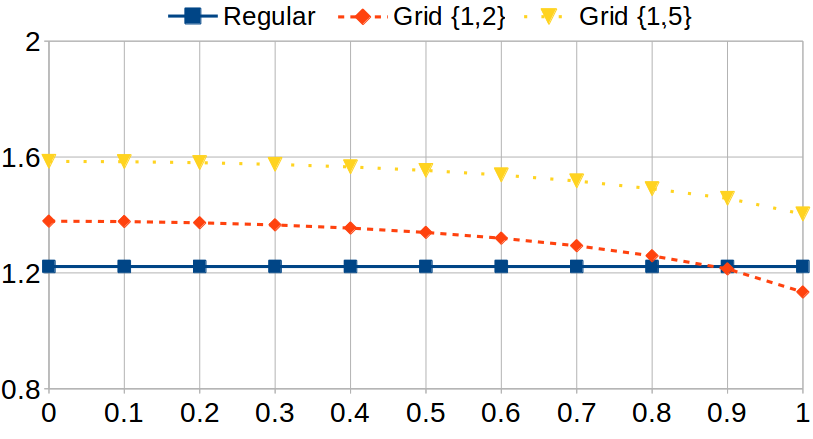
\includegraphics[width=\textwidth]{figures/crowds-mult-2.png}
\caption{$\mathcal{L}_\forall\hyperc{\forall}{C}$, 2 corrupted users.}
\end{subfigure}
\hfill
\centering
\begin{subfigure}[b]{0.45\linewidth}
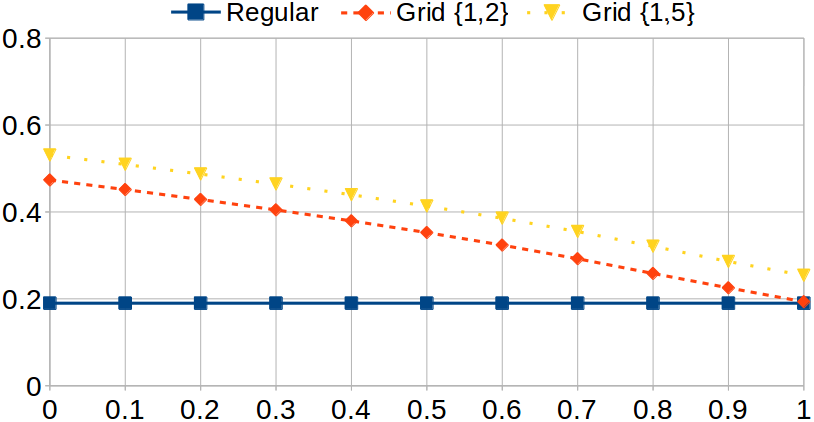
\includegraphics[width=\textwidth]{figures/crowds-add-2.png}
\caption{$\mathcal{L}^+_\forall\hyperc{\pi_u}{C}$, 2 corrupted users.}
\end{subfigure}
\\ \vspace{3mm}
\begin{subfigure}[b]{0.45\linewidth}
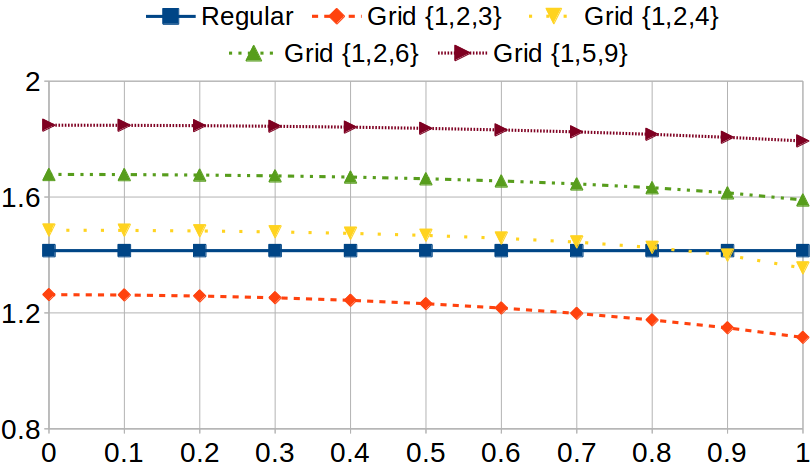
\includegraphics[width=\textwidth]{figures/crowds-mult-3.png}
\caption{$\mathcal{L}_\forall\hyperc{\forall}{C}$, 3 corrupted users.}
\end{subfigure}
\hfill
\centering
\begin{subfigure}[b]{0.45\linewidth}
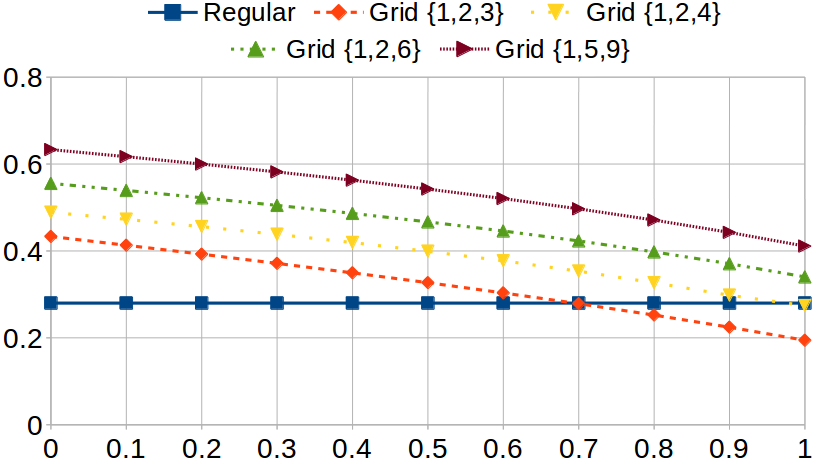
\includegraphics[width=\textwidth]{figures/crowds-add-3.png}
\caption{$\mathcal{L}^+_\forall\hyperc{\pi_u}{C}$, 3 corrupted users.}
\end{subfigure}
%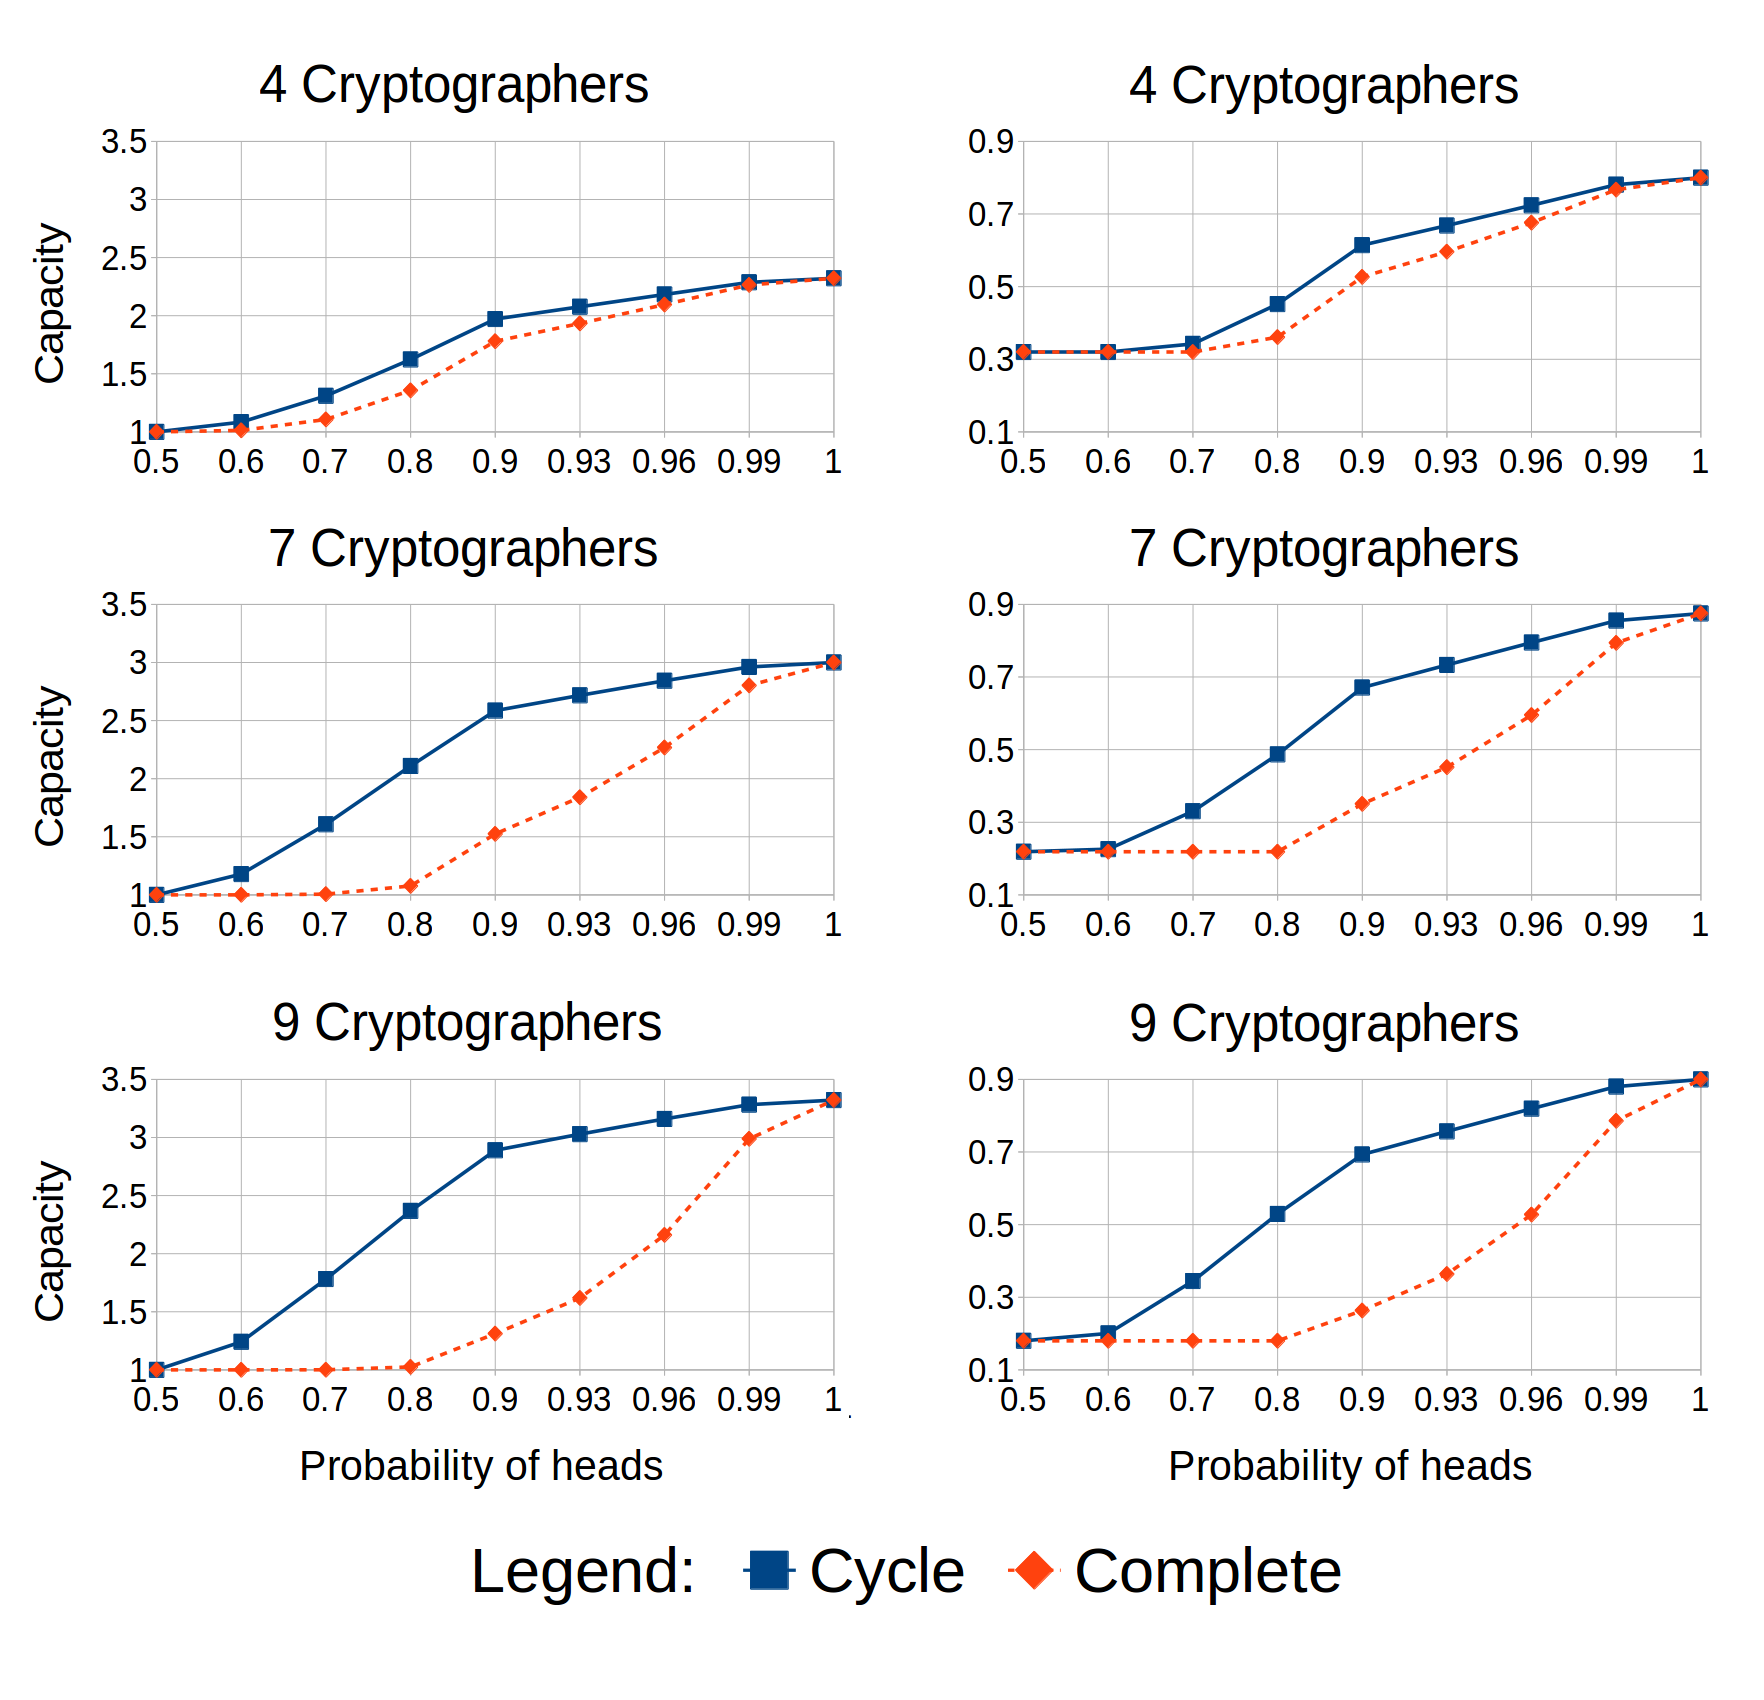
\includegraphics[width=\textwidth]{figures/dining.png}
\caption{Capacities for both variations of Crowds, 
and varying number of corrupt users.
The brackets in the captions indicate positions of corrupt users.}
\label{figure:crgraph}
\end{figure}

As we can verify, the capacities of the channels on the grid variation varies 
considerably according to the position of the corrupt users. 
The results also reiterate our intuition that, for the 3x3 grid with three 
corrupt users, the protocol where 1,2 and 3 are the corrupt users would be the safer one.

It is also interesting to notice that some choice of corrupt users in grid-DC 
actually yield smaller capacities than the original variation.
For 9 users with 3 corrupt ones, for instance, the odds of 
the initiator being detected are 33\%. 
As we have seen, when the corrupt users are 1, 2 and 3 in the
3x3 grid, this chance is 20\%, and our data suggest that this difference is 
sufficient to compensate the extra leakage usually caused by the grid structure.

%\commentA{I have the positions as well. If it is interesting, we can make a deeper 
%analysis on that}

\subsubsection{Results for additive capacity%
%$\mathcal{L}^+_\forall\hyperc{\pi}{C}$
.}

To calculate this capacity, we again use the equation on section~\ref{sec:analdin} and 
consider a uniform prior $\pi_u$. 
The results are shown on Figure~\ref{figure:crgraph}.
%
We can verify that the additive capacities for the original Crowds protocol also 
do not vary with $p_f$.
%\commentA{Should we prove that? It might not be difficult, but it will certainly be quite lengthy}
%\replyM{This could be a cute result for a follow-up paper, maybe a journal version.}
Also, they behave quite differently from their multiplicative counterparts. 
For example, consider again the protocol with 3 corrupt users in positions 1, 2 and 3 
in the 3x3 grid.
The multiplicative capacity of this scenario is always smaller that of the regular protocol, 
but this is not true at all for the additive capacity. 
